
%%******************************************************************************
%% SECTION -•	Métodos 
% Describe the steps you completed during your investigation. This is your
% procedure. Be sufficiently detailed that anyone could read this section and duplicate your experiment. Write it as if you were giving direction for someone else to do the lab. It may be helpful to provide a Figure to diagram your experimental setup.

%%******************************************************************************

\subsection{Métodos}
Os métodos para a elaboração dos testes da eletrônica embarcada são subdivididos
em: planejamento e projeto, desenvolvimento da placa eletrônica, testes da
eletrônica, desenvolvimento de encapsulamento mecânico, montagem e emenda de
cabos submarinos, e teste da integração.

\subsubsection{Planejamento}
O planejamento consiste em avaliar os sensores disponíveis que serão usados na
primeira fase de testes de campo em Jirau. Nesta etapa, há a integração dos
grupos de software e eletrônica para identificar gargalos e tempo hábil para
desenvolvimento de drivers e do hardware para os diversos sensores, protocolos
de comunicação e discutir questões de segurança de equipamento, e facilidade em
manutenção e montagem.

Foi concluído que seria possível obter dados dos seguintes sensores: 
\begin{itemize}
  \item Sonar Micron com comunicação via RS232;
  \item Dois sensores indutivos com saída tipo relé convertida Ethernet;
  \item IMU com saída UART convertida Ethernet;
  \item Profundímetro com saída RS485;
\end{itemize}
Em relação ao Sonar Micron, a eletrônica deve disponibilizar uma saída RS485
de backup para caso a comunicação via RS232 não funcione devido ao comprimento
do cabo 35m.

Os sensores indutivos devem ter sua saída convertida para Ethernet e
backup direto pelo umbilical, caso o driver de comunicação Ethernet não
funcione.

A IMU tem saída UART que é convertida pelo módulo Ethernet. Este sensor
apresenta ainda possibilidade de comunicação RS232, porém com nível lógico TTL
de 5V, o que não é compatível com os conversores RS232-RS485 disponíveis em
laboratório. Como o driver para conversor Ethernet é desenvolvido com
facilidade, não foi realizada a conversão de tensão de 5V-12V para
backup por comunicação RS232.

O profundímetro comunica via RS485, logo um componente MAX485 converte RS485
para UART, a qual é convertida para Ethernet via módulo SCH-remote. O driver,
porém, apresenta maior nível de complexidade. Dessa forma, optou-se por uma
saída extra pelo umbilical, e, na base, há um conversor RS485-USB e o
software Siow em um computador Windows para processar os pacotes recebidos do
sensor.

A alimentação, por questões de possível incompatibilidade com as tensões
disponíveis na usina, pode ser fornecida por um pack de duas baterias 12V ou,
através de um botão, ser fornecida externamente por uma fonte de 24V.

O projeto da placa teste pode ser visto na figura~\ref{fig:prototipo}.

\begin{figure}[H]
 \centering
 \includegraphics[width=1\columnwidth]{EE/figs/prototipo.pdf}
 \caption{Projeto da placa teste}
 \label{fig:prototipo}
 \end{figure}

\subsubsection{Desenvolvimento da placa eletrônica}
Após a elaboração do projeto, uma placa do tipo protoboard foi utilizada para
realizar todas as conexões de alimentação e comunicação.

\begin{figure}[h!]
 \centering
 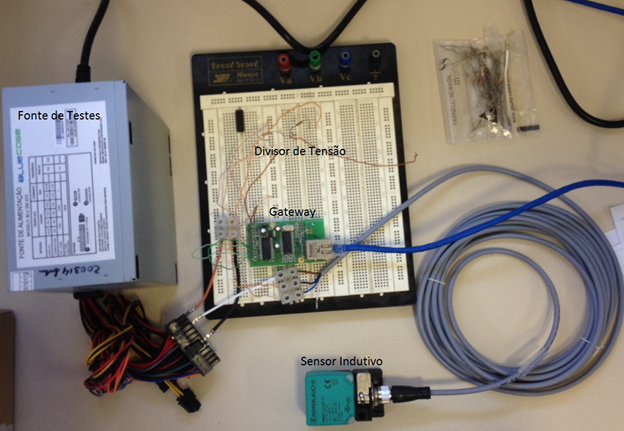
\includegraphics[width=1\columnwidth]{indutivo/figs/indutivo_bancada.png}
 \caption{Eletrônica do sensor indutivo}
 \label{fig:indu_banc}
 \end{figure}


 

\label{metodos}


